\documentclass[10pt]{article}
\usepackage[margin=0.63in]{geometry}
\usepackage[T1]{fontenc}
\usepackage{lmodern,amsmath,amssymb,graphicx,booktabs,hyperref}
\hypersetup{colorlinks=true,urlcolor=blue}
\setlength{\parindent}{0pt}\setlength{\parskip}{5pt}
\begin{document}
\begin{center}{\Large Eight raw sectors, finite aliases and tagged recovery}\\[3pt]
{\small Curve25519 native transport audit --- 24 November 2026}\end{center}

\textbf{Result.} The public-$Q$ wrapper covers eight raw-target sectors and
reconstructs the finite original-map aliases of each returned pair row.
The actual fixed panel has 32 rows over 48 columns, with
$\operatorname{rank}M=\operatorname{rank}[M\mid b]=24$. Its eight kernel
vectors have zero target coefficient, so none gives scalar recovery. The
tiny toy panel recovers its validator scalar 5. These are producer-native
controls, bound by \texttt{PCC-20261124-75bea4}. \texttt{[pcc:unverified]}

\textbf{Original inputs and roles.} Query input is public \texttt{Spec}, $Q$
and a cap; no known scalar, raw lift, multiplier, root list or supplied tuple.
Original parameters $p=2^{255}-19$, $A=486662$, $a=60824497$, $q=213156431$,
$K=20633$, $h$ remain fixed. The parent query derives $h,h^2$ internally.
Output belongs to adapted bases $S_\sigma$, rather than the original fixed
factor base. Actual $Q$ is a public image from the previous known-consistent
fixture, with no scalar supplied relative to RFC $G$. The four tags are
$Q,Q+G,-Q,G$; this is a fixed panel, not a uniform-target cohort.
\texttt{[pcc:unverified]}

\begin{center}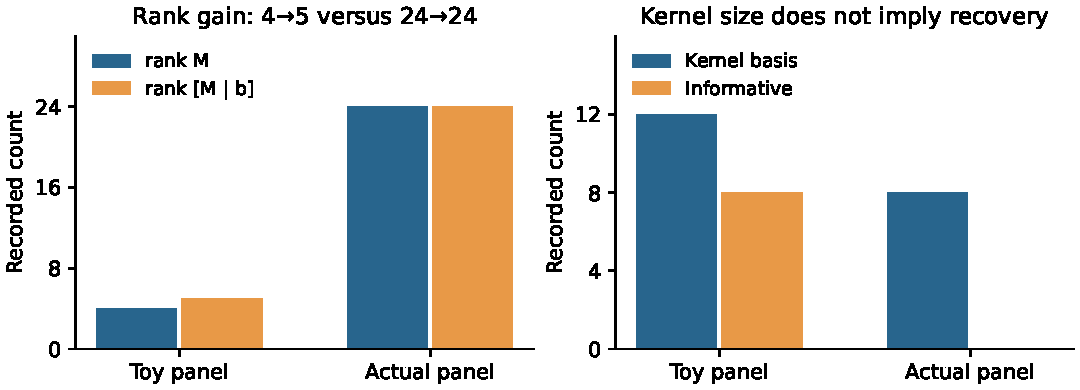
\includegraphics[width=\linewidth]{counts.pdf}\\[-1pt]
{\footnotesize Recorded fixed matrices, native version 1. Four tags in each field;
no statistical interval, timing or growing-size slope is estimated.}\end{center}
\vspace{-6pt}
\begin{center}\small\begin{tabular}{lrrrrrrr}
\toprule
Panel & Rows & Cols & Private & rank $M$ & rank $[M|b]$ & Kernel & Informative\\
\midrule
Toy &16&4&0&4&5&12&8\\
Actual &32&48&32&24&24&8&0\\
\bottomrule
\end{tabular}\end{center}

Known signed $G/Q$ columns are folded into tags before rank. The toy has six
physical columns before that fold; the actual panel has 48. Every toy
informative witness gives 5 and replays in the group. Every actual kernel
vector has $v^Ta=v^Tb=0$, supported on $Q/-Q$ row pairs. Kernel dimension
alone therefore does not establish useful relations. \texttt{[pcc:unverified]}

\textbf{Complete fixed controls.} All 12 nonidentity toy subgroup images,
96 raw sectors, agree with direct full 104-point group and 102-torus pair
enumeration: 284 ordered multiplier/raw lifts. Every finite same-row transport
set matches the union of all-sector roots. The direct reference shares native
field/group/raw-map primitives, so it is separate from factorization but is
not independent signed verification. \texttt{[pcc:unverified]}

The actual targets $Q,Q+G,-Q,G$ return respectively 32,28,32,36 ordered
multiplier/raw lifts and 8,7,8,9 geometric rows. One call completes all four
planned groups: 16 public-$Q$ queries, 128 parent sector calls, 35 records,
exit 0. Nine guard refusals and private/duplicate/signed/informative synthetic
linear controls are retained. Wrong target tags reject in the group before
rank. Caps are incomplete errors, not absence certificates.
\texttt{[pcc:unverified]}

\newpage
\begin{center}{\large Construction, exact scope and next discriminator}\end{center}
\begin{center}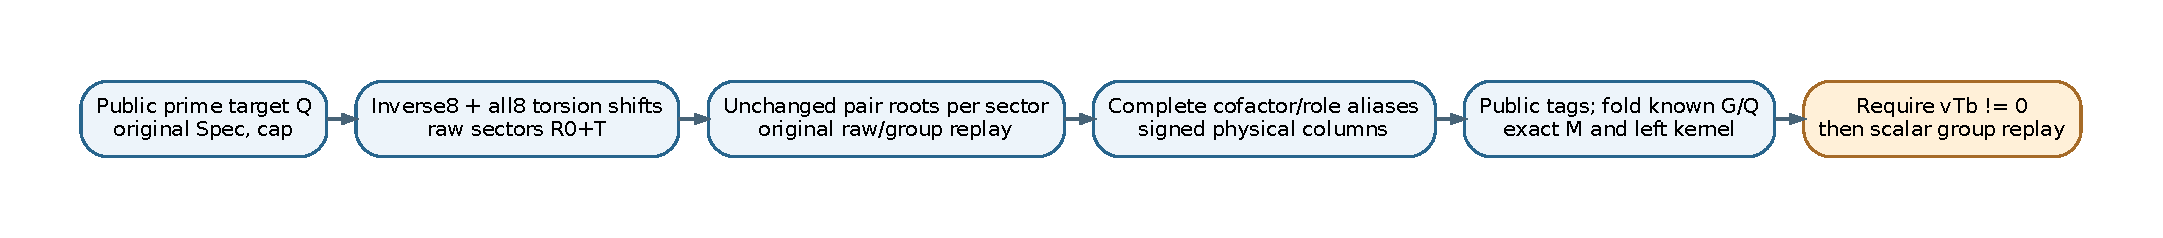
\includegraphics[width=\linewidth]{diagram.pdf}\end{center}

\textbf{Torsion sectors and finite aliases.} For a nonzero prime-subgroup
target, set $R_0=[8^{-1}\bmod\ell]Q$. Under the original order-$8\ell$
rational-group hypotheses, every raw target is $R_0+T$, $T\in E(\mathbb F_p)[8]$.
The component derives an order-eight generator, checks eight distinct points
and replays their images; each sector invokes the unchanged pair root solver.
For a raw point $(x,y)$, the original map rearranges to
\[
 \tau=\frac{\epsilon A}{2x+A},\qquad
 \eta^2=\frac{\tau^2-1}{2},\qquad \epsilon\in\{1,-1\}.
\]
Each candidate still passes norm/chart and original unique-rational-branch
admission \emph{before} zero/torsion filtering. The written conditional bound
is at most 32 encodings per image and 64 role candidates in union. Intersect
both role assignments, retain raw provenance and replay exact sums. This
is finite alias transport, not a formal native group/map or logarithm-transport
theorem. \texttt{[pcc:unverified]}

\textbf{Recovery criterion.} Normalize signed physical columns; retain public
target tags in $Mz=a+bx$. Exact subgroup-field elimination records invertible
row operations and checks their replay and every left-kernel product.
An informative witness must satisfy
\[
 v^TM=0,\quad v^Tb\ne0,\quad x=-\frac{v^Ta}{v^Tb},\quad [x]G=Q.
\]
The actual recorded matrix fails that benefit gate. This closes only the
predeclared panel's useful-linear-recovery test. It does not reject every
cofactor method, adaptive base, nonlinear algorithm or index-calculus route.
\texttt{CRITERIA.md} preserves that distinction. \texttt{[pcc:unverified]}

\textbf{Formal fidelity.} \texttt{PCC-20261124-8b98c4} binds two concrete Nat
inverse-eight Bezout obligations. Focused project gate: two named, zero
failing, zero trusted; those endpoints use no axioms. Anonymous Mathlib
homomorphism probes are separate. Native curve/field/group equivalence,
kernel cardinality, map refinement and certificate-checker soundness remain
open. Evaluated degree-three identity \texttt{IDC1hec732500b4efd748} has 32+32
format-field points and plus-one refusal; it is not a formal native inverse
proof. See \texttt{PROOF\_MAP.md}. \texttt{[pcc:unverified]}

\textbf{Source and execution custody.} Four release unit tests, formatting,
strict all-target Clippy and build passed before qualification. Source
\texttt{ee1a401f1f} published as \texttt{f1f9348521} before the single call:
111 native inputs, five constituent archives, six compiled hashes.
The retained 1805520-byte binary has SHA-256 prefix
\texttt{f0a0b1d261aefbd4f3b7}.\\
Distinct build/pre/post, copied immutable
qualifier, actual wrapper transport and separate stdout are retained. No
qualified source edit or test/worker rerun followed. All standing is producer
unsigned. No GAE, timing, RSS, complete cold cost, fastest-tool or exponent
claim follows from these correctness records. \texttt{[pcc:unverified]}

\textbf{Publication.} Full raw 1708591 bytes is in one lossless 140084-byte,
28-member archive.\\
SHA-256 prefix \texttt{f86428a9b3762ed56133}. Actual policy
selects it for storage. It is staged at its canonical path for trusted
artifact-autofix; a real upload/replay receipt remains required. Local
transport installation succeeded, but caller credentials are unavailable.
No invented receipt, policy exemption or remote deletion.
\texttt{[pcc:unverified]}

\textbf{Next.} Bound fixed-template target incidence before more equality-only
queries. Then specify a growing ratio family or genuine non-torsion transport
with original-root correspondence, cold search costs and informative tags.
All original yield/family/private-selection/kernel/recovery criteria remain.
No successor campaign is scheduled by the CI checker. Sources checked:
RFC7748 section 4.1; RFC9380 sections 6.7.1/7; Ristretto quotient context;
Zaslavsky sections III--IV (simple graphs only); previous original map/criteria.
KB wrapper unavailable. No novelty for those classical methods; canonical
performance graphs have no new admitted row. \texttt{[pcc:unverified]}
\end{document}
